\newpage
\subsection{Μελέτη του BTB}
\vspace{3mm}

Στο σημείο αυτό μελετάμε την απόδοση του BTB για διαφορες τιμές entries. 
Συγκεκριμένα έχουμε τους εξής συνδυασμούς:
\begin{itemize}
   \item 512 lines, associativity 1 
   \item 256 lines, associativity 2 
   \item 128 lines, associativity 4 
   \item 64 lines, associativity 8 
   \item 32 lines, associativity 4 
   \item 8 lines, associativity 8 
\end{itemize}

\vspace{1em}
Ακολουθούν τα διαγράμματα και ο σχετικός σχολιασμός:\vspace{1em}
\vspace{1em}    

   \begin{minipage}{\textwidth}
      \begin{center}
         \fbox{\textlatin{\textbf{\textit{403-gcc}}}}\\
         \vspace{3mm}
         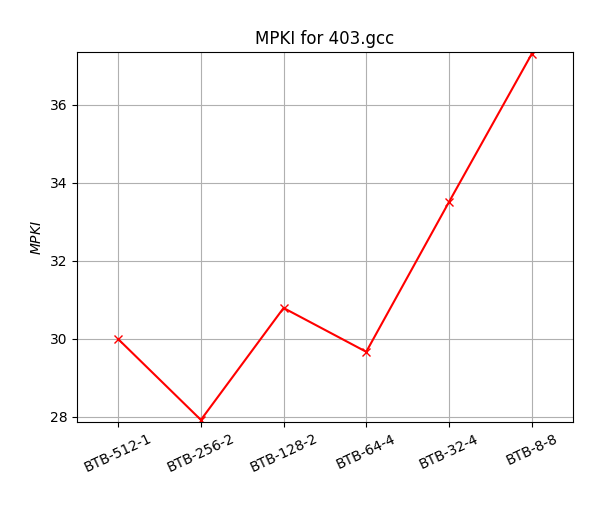
\includegraphics[width=0.65\textwidth, frame]{./graphs/4-3/403-gcc.png}
         \vspace{6mm}
      \end{center}
   \end{minipage}

   \begin{minipage}{\textwidth}
      \begin{center}
         \fbox{\textlatin{\textbf{\textit{429-mcf}}}}\\
         \vspace{3mm}
         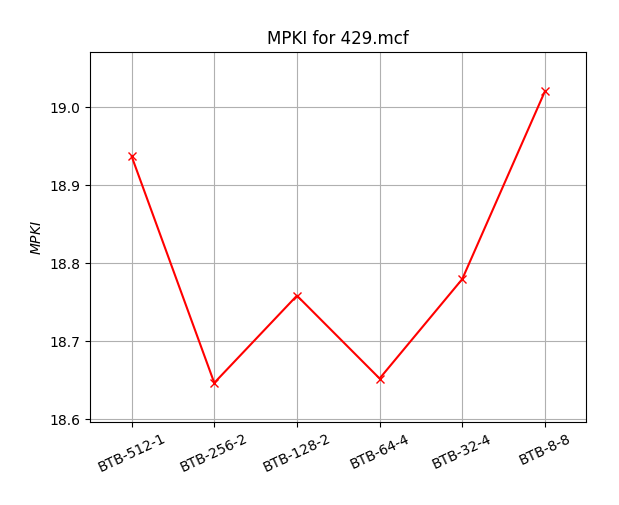
\includegraphics[width=0.65\textwidth, frame]{./graphs/4-3/429-mcf.png}
         \vspace{6mm}
      \end{center}
   \end{minipage}

   \begin{minipage}{\textwidth}
      \begin{center}
         \fbox{\textlatin{\textbf{\textit{434-zeusmp}}}}\\
         \vspace{3mm}
         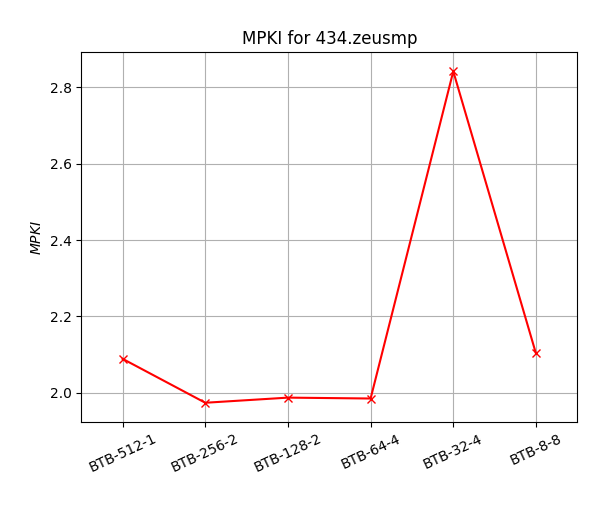
\includegraphics[width=0.65\textwidth, frame]{./graphs/4-3/434-zeusmp.png}
         \vspace{6mm}4
      \end{center}
   \end{minipage}

   \begin{minipage}{\textwidth}
      \begin{center}
         \fbox{\textlatin{\textbf{\textit{436-cactusADM}}}}\\
         \vspace{3mm}
         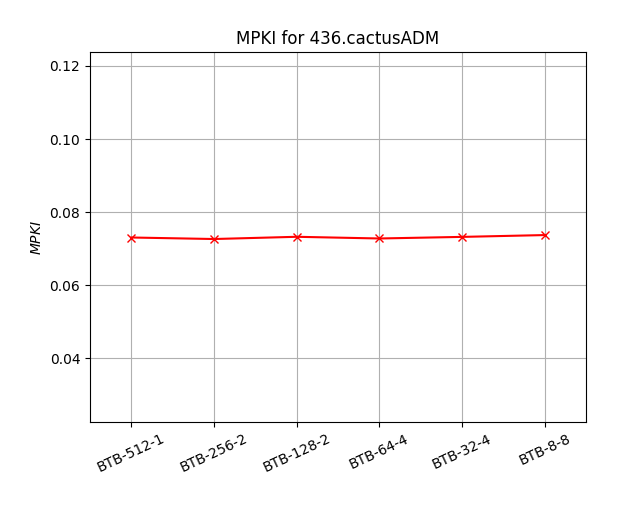
\includegraphics[width=0.65\textwidth, frame]{./graphs/4-3/436-cactusADM.png}
         \vspace{6mm}
      \end{center}
   \end{minipage}

   \begin{minipage}{\textwidth}
      \begin{center}
         \fbox{\textlatin{\textbf{\textit{445-gobmk}}}}\\
         \vspace{3mm}
         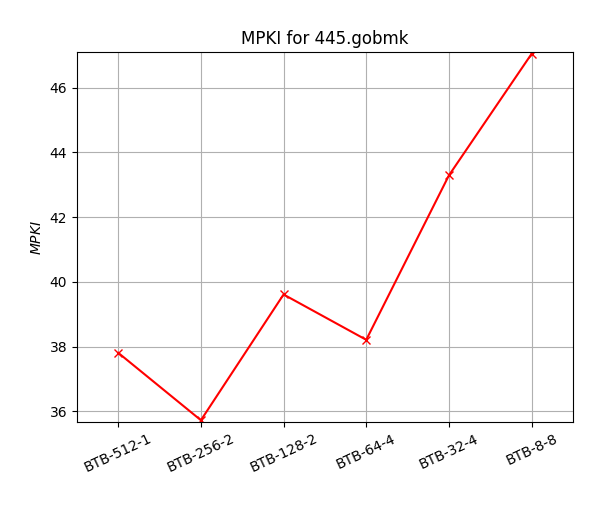
\includegraphics[width=0.65\textwidth, frame]{./graphs/4-3/445-gobmk.png}
         \vspace{6mm}
      \end{center}
   \end{minipage}

   \begin{minipage}{\textwidth}
      \begin{center}
         \fbox{\textlatin{\textbf{\textit{450-soplex}}}}\\
         \vspace{3mm}
         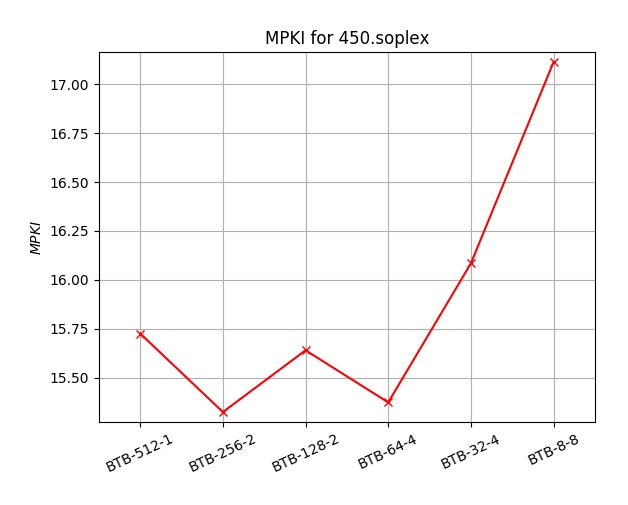
\includegraphics[width=0.65\textwidth, frame]{./graphs/4-3/450-soplex.png}
         \vspace{6mm}
      \end{center}
   \end{minipage}

   \begin{minipage}{\textwidth}
      \begin{center}
         \fbox{\textlatin{\textbf{\textit{456-hmmer}}}}\\
         \vspace{3mm}
         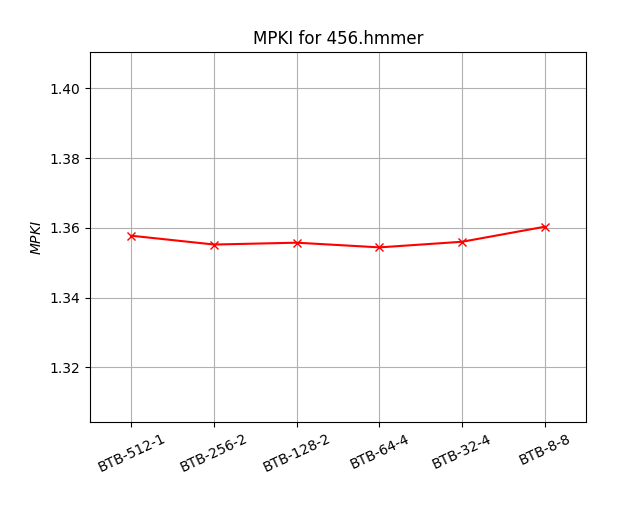
\includegraphics[width=0.65\textwidth, frame]{./graphs/4-3/456-hmmer.png}
         \vspace{6mm}
      \end{center}
   \end{minipage}

   \begin{minipage}{\textwidth}
      \begin{center}
         \fbox{\textlatin{\textbf{\textit{458-sjeng}}}}\\
         \vspace{3mm}
         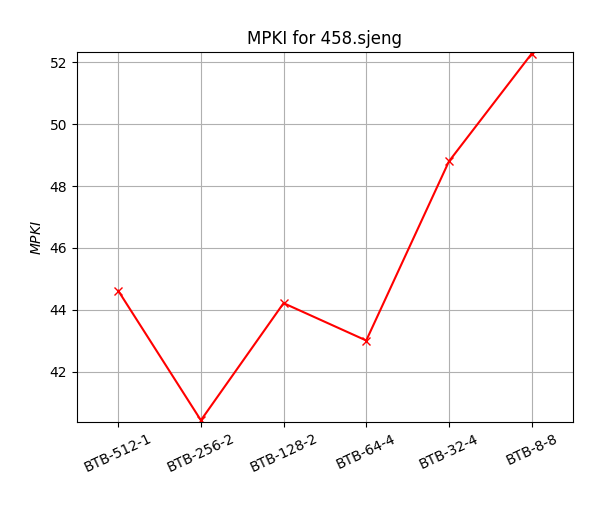
\includegraphics[width=0.65\textwidth, frame]{./graphs/4-3/458-sjeng.png}
         \vspace{6mm}
      \end{center}
   \end{minipage}

   \begin{minipage}{\textwidth}
      \begin{center}
         \fbox{\textlatin{\textbf{\textit{459-GemsFDTD}}}}\\
         \vspace{3mm}
         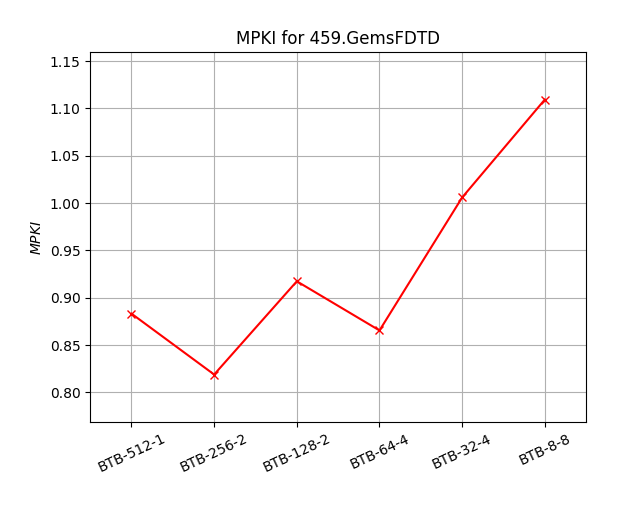
\includegraphics[width=0.65\textwidth, frame]{./graphs/4-3/459-GemsFDTD.png}
         \vspace{6mm}
      \end{center}
   \end{minipage}

   \begin{minipage}{\textwidth}
      \begin{center}
         \fbox{\textlatin{\textbf{\textit{471-omnetpp}}}}\\
         \vspace{3mm}
         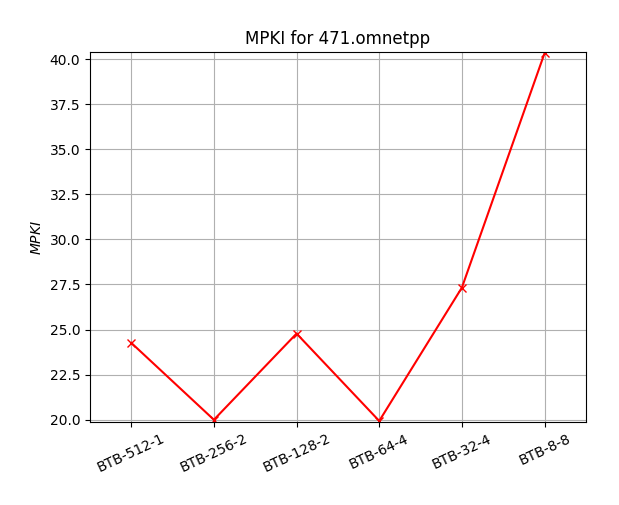
\includegraphics[width=0.65\textwidth, frame]{./graphs/4-3/471-omnetpp.png}
         \vspace{6mm}
      \end{center}
   \end{minipage}

   \begin{minipage}{\textwidth}
      \begin{center}
         \fbox{\textlatin{\textbf{\textit{473-astar}}}}\\
         \vspace{3mm}
         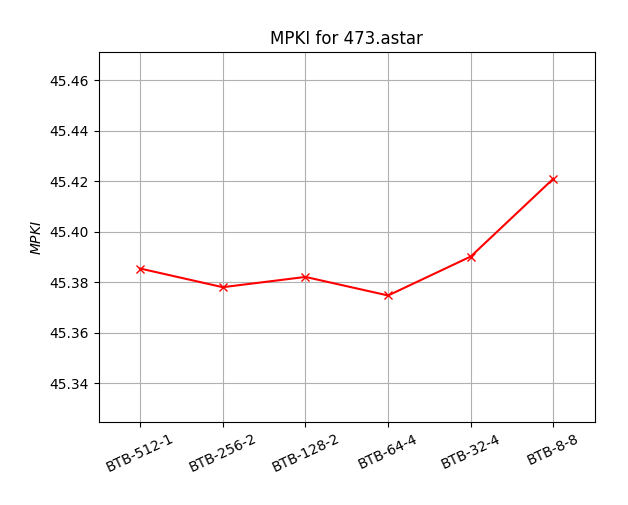
\includegraphics[width=0.65\textwidth, frame]{./graphs/4-3/473-astar.png}
         \vspace{6mm}
      \end{center}
   \end{minipage}

   \begin{minipage}{\textwidth}
      \begin{center}
         \fbox{\textlatin{\textbf{\textit{483-xalancbmk}}}}\\
         \vspace{3mm}
         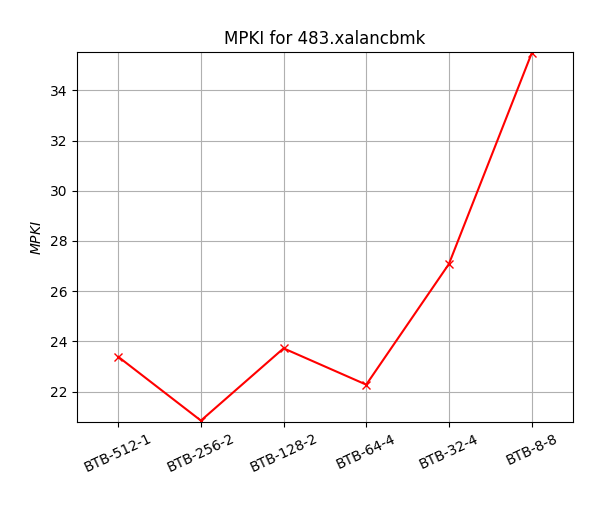
\includegraphics[width=0.65\textwidth, frame]{./graphs/4-3/483-xalancbmk.png}
         \vspace{6mm}
      \end{center}
   \end{minipage}

   \begin{minipage}{\textwidth}
      \begin{center}
         \fbox{\textlatin{\textbf{\textit{Geometric Average of MPKI}}}}\\
         \vspace{3mm}
         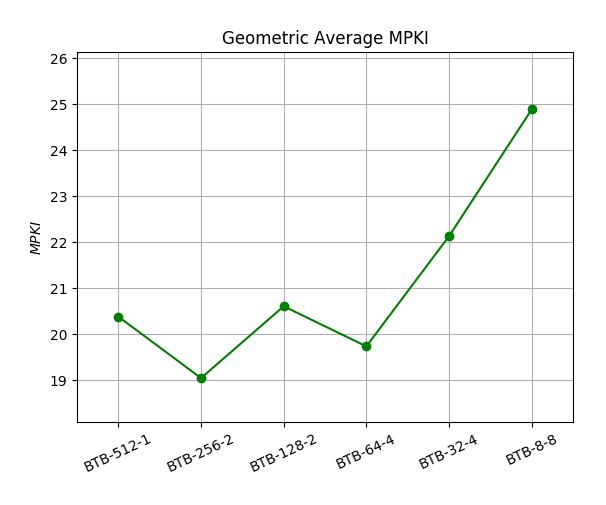
\includegraphics[width=0.65\textwidth, frame]{./graphs/4-3/mean.png}
         \vspace{6mm}
      \end{center}
   \end{minipage}


   \begin{minipage}{\textwidth}
      \begin{center}
         \fbox{\textlatin{\textbf{\textit{Benchmarks Overview}}}}\\
         \vspace{3mm}
         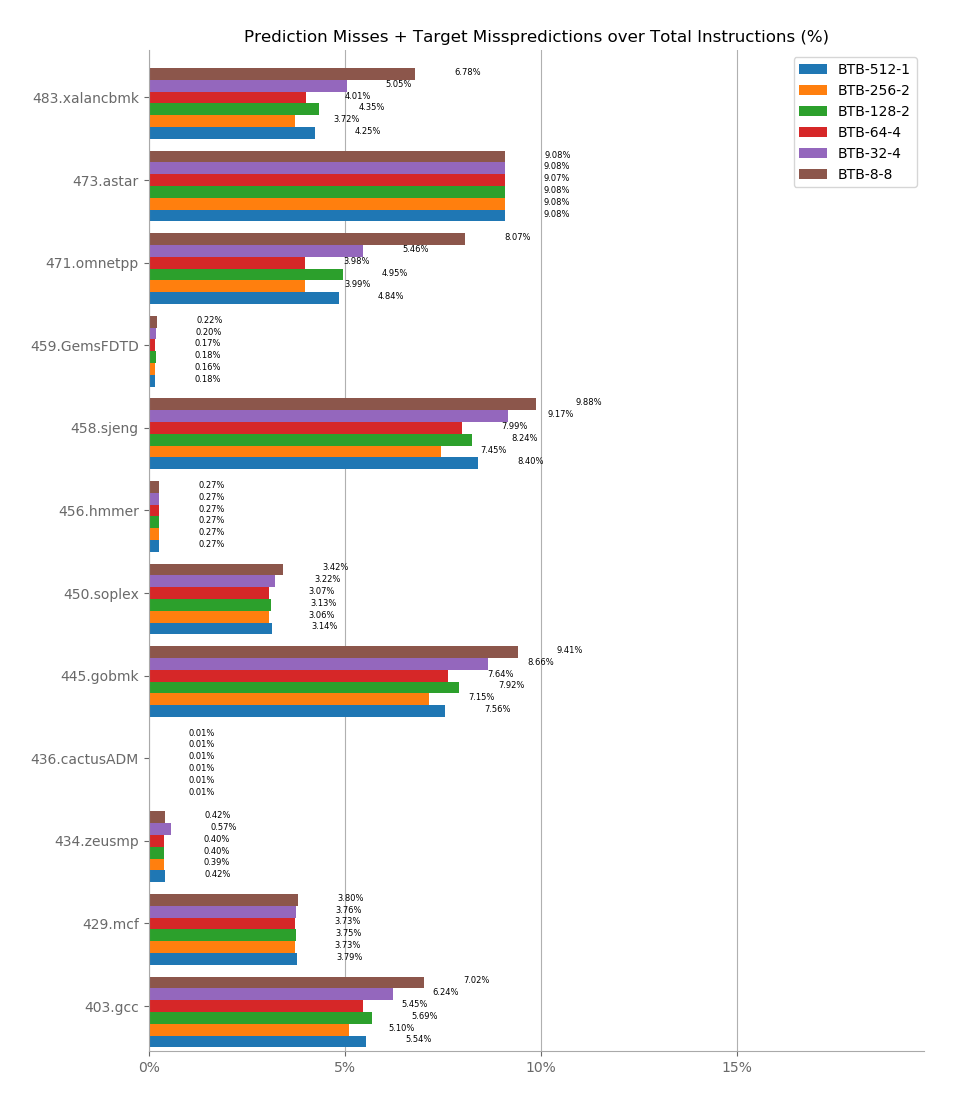
\includegraphics[width=\textwidth, frame]{./graphs/4-3/bar_chart.png}
         \vspace{6mm}
      \end{center}
   \end{minipage}

\paragraph{Συμπεράσματα-Σχόλια}
   Στα παραπάνω διαγράμματα χρησιμοποιούμε ως μετρική τα επιμέρους prediction misses +
   target misspredictions per KILOInstructions.

   Από τα επιμέρους διαγράμματα διαπιστώνουμε ότι για σταθερό πλήθος entries
   (table lines x associativity) η αύξηση του associativity επιφέρει βελτίωση.
   Την μιρκότερη τιμή misses επιτυγχάνουν οι συνδυασμοί BTB-256-2 και BTB-64-4.
   Μάλιστα ο BTB-256-2 φαίνεται να έχει καθολικό προβάδισμα στην απόδοση όπως
   βλέπουμε και στο διάγραμμα των γεωμετρικών μέσων. 

   Αξίζει να σημειώσουμε πως ο συνδυασμός BTB-8-8 έχει τη χειρότερη απόδοση, και
   άρα η υπερβολική αύξηση του associativity μειώνοντας τα table lines μετά από
   ένα όριο δε δρα βελτιωτικά.
  
   Τέλος από το ραβδόγραμμα Benchmarks Overview, όπου φαίνονται συγκεντρωτικά
   όλα τα παραπάνω και παρουσιάζονται τα total misspredictions per total
   instructions (\%), μπορούμε να επιβεβαιώσουμε ξανά ότι o BTB-256-2 έχει την
   καλύτερη επίδοση. Να σημειώσουμε σε αυτό το σημείο ότι στο διάγραμμα αυτό
   κάποια μετροπρογράμματα φαίνονται να έχουν υπερβολικά κάλή επίδοση (hmmer,
   cactusADM, etc), όμως αυτό οφείλεται εν μέρει και στο ότι γενικότερα έχουν
   μιρκό ποσοστό branches, όπως είδατε στο πρώτο τμήμα της παρούσας άσκησης.
   
   \textbf{Συνοπτικά, καλύτερη επιλογή είναι ο BTB Predictor με 512 entries, οργανωμένα σε 256 lines και associativity 2. }.

